% % LLNCS macro package for Springer Computer Science proceedings;
% Version 2.21 of 2022/01/12
%
\documentclass[runningheads]{llncs}
%
\usepackage[T1]{fontenc}
% T1 fonts will be used to generate the final print and online PDFs,
% so please use T1 fonts in your manuscript whenever possible.
% Other font encondings may result in incorrect characters.
%

\usepackage{amsmath}
\usepackage{todonotes}

\usepackage[left=2cm,
            right=2cm,
            top=2cm,
            bottom=2cm]{geometry}

\usepackage{graphicx, color, float, subfig}
\captionsetup{font=small,labelfont=bf,labelsep=period,skip=5pt}
\captionsetup[subfloat]{font=scriptsize,labelfont=bf,skip=5pt}

%
\usepackage{hyperref}
\renewcommand\UrlFont{\color{blue}\rmfamily}
\urlstyle{rm}
%

\begin{document}
\title{\fontsize{12}{12}\selectfont Project 1 - Cat \& Dog Classification}
\titlerunning{Project 1}
%
\author{Henrik Daniel Christensen\orcidID{hench13@student.sdu.dk} \\Frode Engtoft Johansen\orcidID{fjoha21@student.sdu.dk}}
\authorrunning{Christensen, Johansen} % first names are abbreviated in the running head.
%
\institute{DM873: Deep Learning\\University of Southern Denmark, SDU\\\textit{Department of Mathematics and Computer Science}}
%
\maketitle % typeset the header of the contribution

%%%%%%%%%%%%%%%%%%%%%%%%%%%%%%%%%%%%%%%%%%%
\section{Introduction}
The objective of this project is to develop a deep learning model capable of distinguishing between images of cats and dogs.
The task involves training a neural network using a dataset containing 3,600 images, equally divided between the two categories.

% The report is structured as follows: Section 2 explores the dataset and the possible features that can be extracted from it.
% Section 3 describes which data augmentation techniques were used for the model training.
% Section 4 presents the architecture of the neural network.
% Section 5 describes the training process used to optimize the model.
% Section 6 presents the results obtained by the model.
% Section 7 presents the results of using a pre-trained model. Section 8 discusses the results and the limitations of the model.
% Finally, Section 9 concludes the report.
% In the Appendix, the code and a notebook with the results and visualizations are provided.
\section{Explorative Analysis}
\begin{figure}[H]
    \vspace*{-0.7cm}
    \centering
    \subfloat[][Cats]{%
        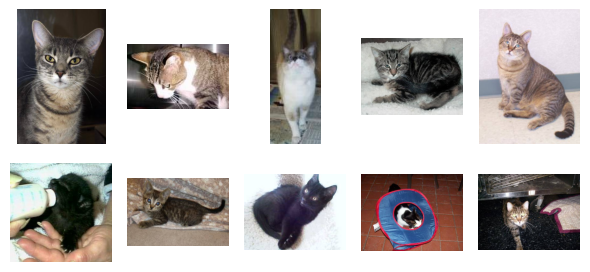
\includegraphics[width=0.35\textwidth]{figures/cats.png}\label{fig:cats}}\hspace{1cm}
    \subfloat[][Dogs]{%
        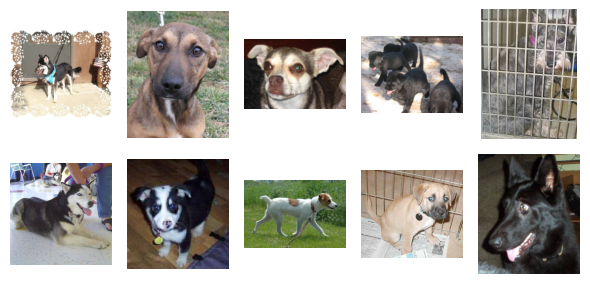
\includegraphics[width=0.35\textwidth]{figures/dogs.png}\label{fig:dogs}}
    \caption{Illustration of the effect of adaptive grids.}
    \label{fig:cats_dogs}
    \vspace*{-0.7cm}
\end{figure}

Dataset contains many diverse images and differ in terms of color, size, and orientation. The images are of varying quality, with some being clear and well-lit, while others are blurry or poorly framed. The dataset contains a mix of close-up shots and full-body shots of both cats and dogs. The dataset contains a mix of different breeds of cats and dogs, with varying fur lengths, colors, and patterns. Most of the pictures are 220-500 pixels wide, and 220-500 pixels tall. They are all in color, so they have 3 color channels. 

Cats vs. Dogs features
- Face:
- Cats generally have shorter, more rounded faces, often with triangular ears and pointed noses.
- Dogs generally have longer snouts and a greater diversity in ear shapes.
- Ears:
- Cats ears are typically upright and pointed.
- Dogs ears vary widely in shape and position, from erect to floppy, and they often have a different positioning on the head compared to cats.
- Eyes:
- Cats have generally more sharper-shaped eyes.
- Dogs have rounder eyes.
- Tail:
- Cats have long, flexible tails, often held upright or curled.
- Dogs’ tails vary greatly in length and shape, often held in different positions.
- Body Structure:
- Cats are generally lean, with flexible, agile bodies.
- Dogs come in a range of body types, from muscular to slender.
- Fur and Markings:
- Cats fur are often softer, finer, and smoother.
- Dogs often are coarser.
\section{Base Model}
First, we set out to develop a base model. However, first, we had to decide which image size to use.
We chose an image size of 224 by 224, since almost all images are bigger on each axis, so we almost only shrink pictures.
The pretrained models also uses resizing to 224 pixels making our model more comparable to the pretrained ones.
Resizing the images has the effect of reducing the size of the input to the model which will reduce the accuracy a little bit, but make it train significantly faster.

Next, we had to decide how many layers our model should have.
As the task is relatively simple, we decided to use 4 convolutional layers and 3 fully connected layers.
The base model is shown in Table \ref{tab:base_model}.
\begin{table}[H]
    \vspace*{-0.5cm}
    \centering
    \begin{tabular}{|l|c|c|c|c|}
    \hline
                & \textbf{Output}           & \textbf{Kernel}   & \textbf{MaxPooling}   & \textbf{Activation}   \\ 
                & \textbf{kernels/features} &                   &   &   \\ \hline
    Conv2D w/   & 32                        & 3x3                   & 2x2                   & ReLU                  \\ \hline
    Conv2D w/   & 64                        & 3x3                   & 2x2                   & ReLU                  \\ \hline
    Conv2D w/   & 128                       & 3x3                   & 2x2                   & ReLU                  \\ \hline
    Conv2D w/   & 256                       & 3x3                   & 2x2                   & ReLU                  \\ \hline
    Linear w/   & 256                       & -                     & -                     & ReLU                  \\ \hline
    Linear w/   & 128                       & -                     & -                     & ReLU                  \\ \hline
    Linear w/   & 2                         & -                     & -                     & -                     \\ \hline
    \end{tabular}
    \caption{Base Model.}
    \label{tab:base_model}
    \vspace*{-0.8cm}
\end{table}
Results of the base model after 25 epochs are shown in Figure \ref{fig:base_model_results}.
% \begin{figure}[H]
    %     \vspace*{-0.7cm}
    %     \centering
    %     \includegraphics[width=0.8\textwidth]{figures/pretrained_model_results.png}
    %     \caption{Base Model Results.}
    %     \label{fig:base_model_results}
    %     \vspace*{-0.7cm}
    % \end{figure}

Clearly, the base model is overfitting, one way, especially for small datasets as in this case, to reduce overfitting is to use data augmentation, enabling the model to learn from more data.
\section{Regularization}

\subsection{Data Augmentation}
We chose to augment the data in a few different ways since we want to generalize the data so the important features remain. 
Using augmentation ensures that it will get better accuracy when faced with new images. In other words, it reduces overfitting.

The images are of varying quality and taken in different lighting, and this is also what we can expect from the final test set.
For this reason we change the brightness, saturation, and contrast. Furthermore, the pictures are taken from different angles so we rotate the pictures slightly and flip them horizontally. Generally, images of animals are not vertically flipped, so we chose not to do this, but of course, some cases may exist.

The pictures are also cropped differently to get finer details from the images, as well as the images becomes scale invariant.

Even though some of the pictures are more blurry than others, we chose to not use blurring as data augmentation, as it effectively just reduces the data of the image without reducing input to the model.

We shear and translate the pictures to emulate pictures taken from different angles of the animal.

Since the training dataset is quite small, we wanted to create more data by reusing the same images but with random augmentations, but in the end we found out that our results did not improve from this.


Many different data augmentation techniques exists, to find the best data augmentation techniques for this task, one image was used to test different techniques.



The techniques used for this task as well as augmented sample images by these techniques are shown in Figure \ref{fig:augmentation}.

\begin{figure}[H]
    \vspace*{-0.7cm}
    \centering
    \subfloat[Data Augmentation Techniques.\label{tab:augmentation}]{
        \raisebox{\height}{ % align at the bottom
        \begin{tabular}{|l|p{2.8cm}|}
            \hline
            \textbf{Data Augmentation} & \textbf{Parameters} \\ \hline
            RandomHorizontalFlip & 50\% \\ \hline
            ColorJitter & brightness=0.2 \newline contrast=0.2 \newline saturation=0.2 \newline hue=0 \\ \hline
            RandomAffine & degrees=25 \newline translate=(0.1, 0.1) \newline scale=(0.7, 1.3) \newline shear=(-10, 10) \\ \hline
        \end{tabular}}}
    \hspace{0.4cm}
    \subfloat[Sample images after augmentation.\label{fig:augmentation_images}]{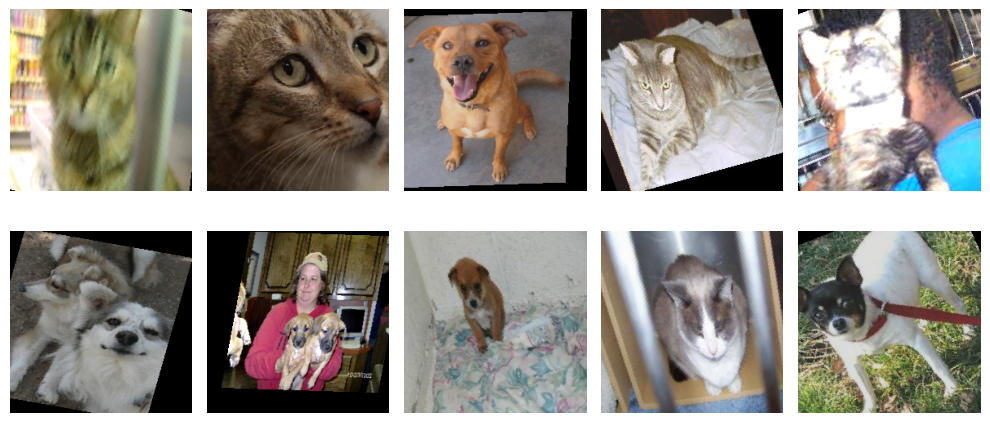
\includegraphics[width=0.5\textwidth]{figures/augmentation.png}}
    \caption{Data augmentation techniques.}
    \label{fig:augmentation}
    \vspace*{-0.7cm}
\end{figure}


\begin{figure}[H]
    \centering
    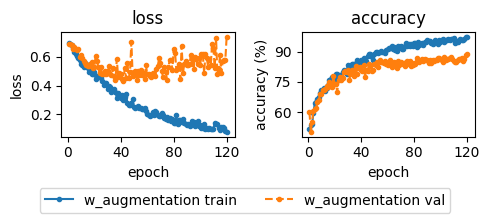
\includegraphics[width=0.4\textwidth]{figures/results_augmentation.png}
    \caption{Sample images after augmentation.}
    \label{fig:augmentation_results}
\end{figure}


\subsection{More Regularization Techniques}


1:
- 93% valideringsæt
- 84% test

2:
- 93% valideringsæt
- 85% test sæt

- loss mere stabil på 2. Den er med weight decay og halvering af learning rate hver 25 epoker.
- dropout layer

\begin{figure}[H]
    \vspace*{-0.7cm}
    \centering
    \subfloat[Regularized model 1.\label{fig:reg1}]{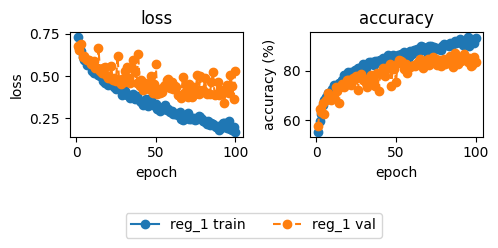
\includegraphics[width=0.4\textwidth]{figures/results_reg_1.png}}
    \hspace{1cm}
    \subfloat[Regularized model 2.\label{fig:reg2}]{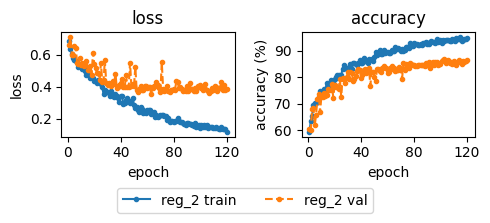
\includegraphics[width=0.4\textwidth]{figures/results_reg_2.png}}
    \caption{Results using regularization.}
    \label{fig:reg}
    \vspace*{-0.7cm}
\end{figure}

\subsection{Adding one more convolutional layer}
\begin{figure}[H]
    \vspace*{-0.7cm}
    \centering
    \subfloat[Regularized model 3.\label{fig:reg1}]{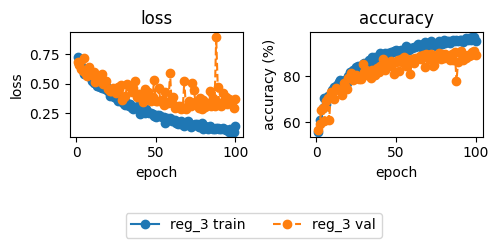
\includegraphics[width=0.4\textwidth]{figures/results_reg_3.png}}
    \hspace{1cm}
    \subfloat[Regularized model 4.\label{fig:reg2}]{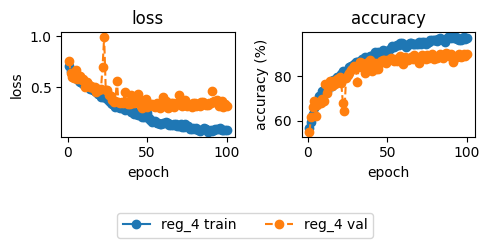
\includegraphics[width=0.4\textwidth]{figures/results_reg_4.png}}
    \caption{Results using one more convolutional layer.}
    \label{fig:reg}
    \vspace*{-0.7cm}
\end{figure}
\section{Prediction}
For prediction on the test set, we choose the model 'Regularized model 4' as it achieves the highest validation accuracy.
The model is applied to the test set, with its accuracy result summarized in Table \ref{tab:prediction}.

\begin{table}[H]
    \centering
    \begin{tabular}{|c|c|}
        \hline
        \textbf{Test Accuracy using Reg4 model} \\ \hline
        91.5\% \\ \hline
    \end{tabular}
    \caption{Test Accuracy using Reg4 Model.}
    \label{tab:prediction}
\end{table}

Some of the misclassified and correctly classified images are given in Figure \ref{fig:prediction}.
\begin{figure}[H]
    \vspace*{-0.7cm}
    \centering
    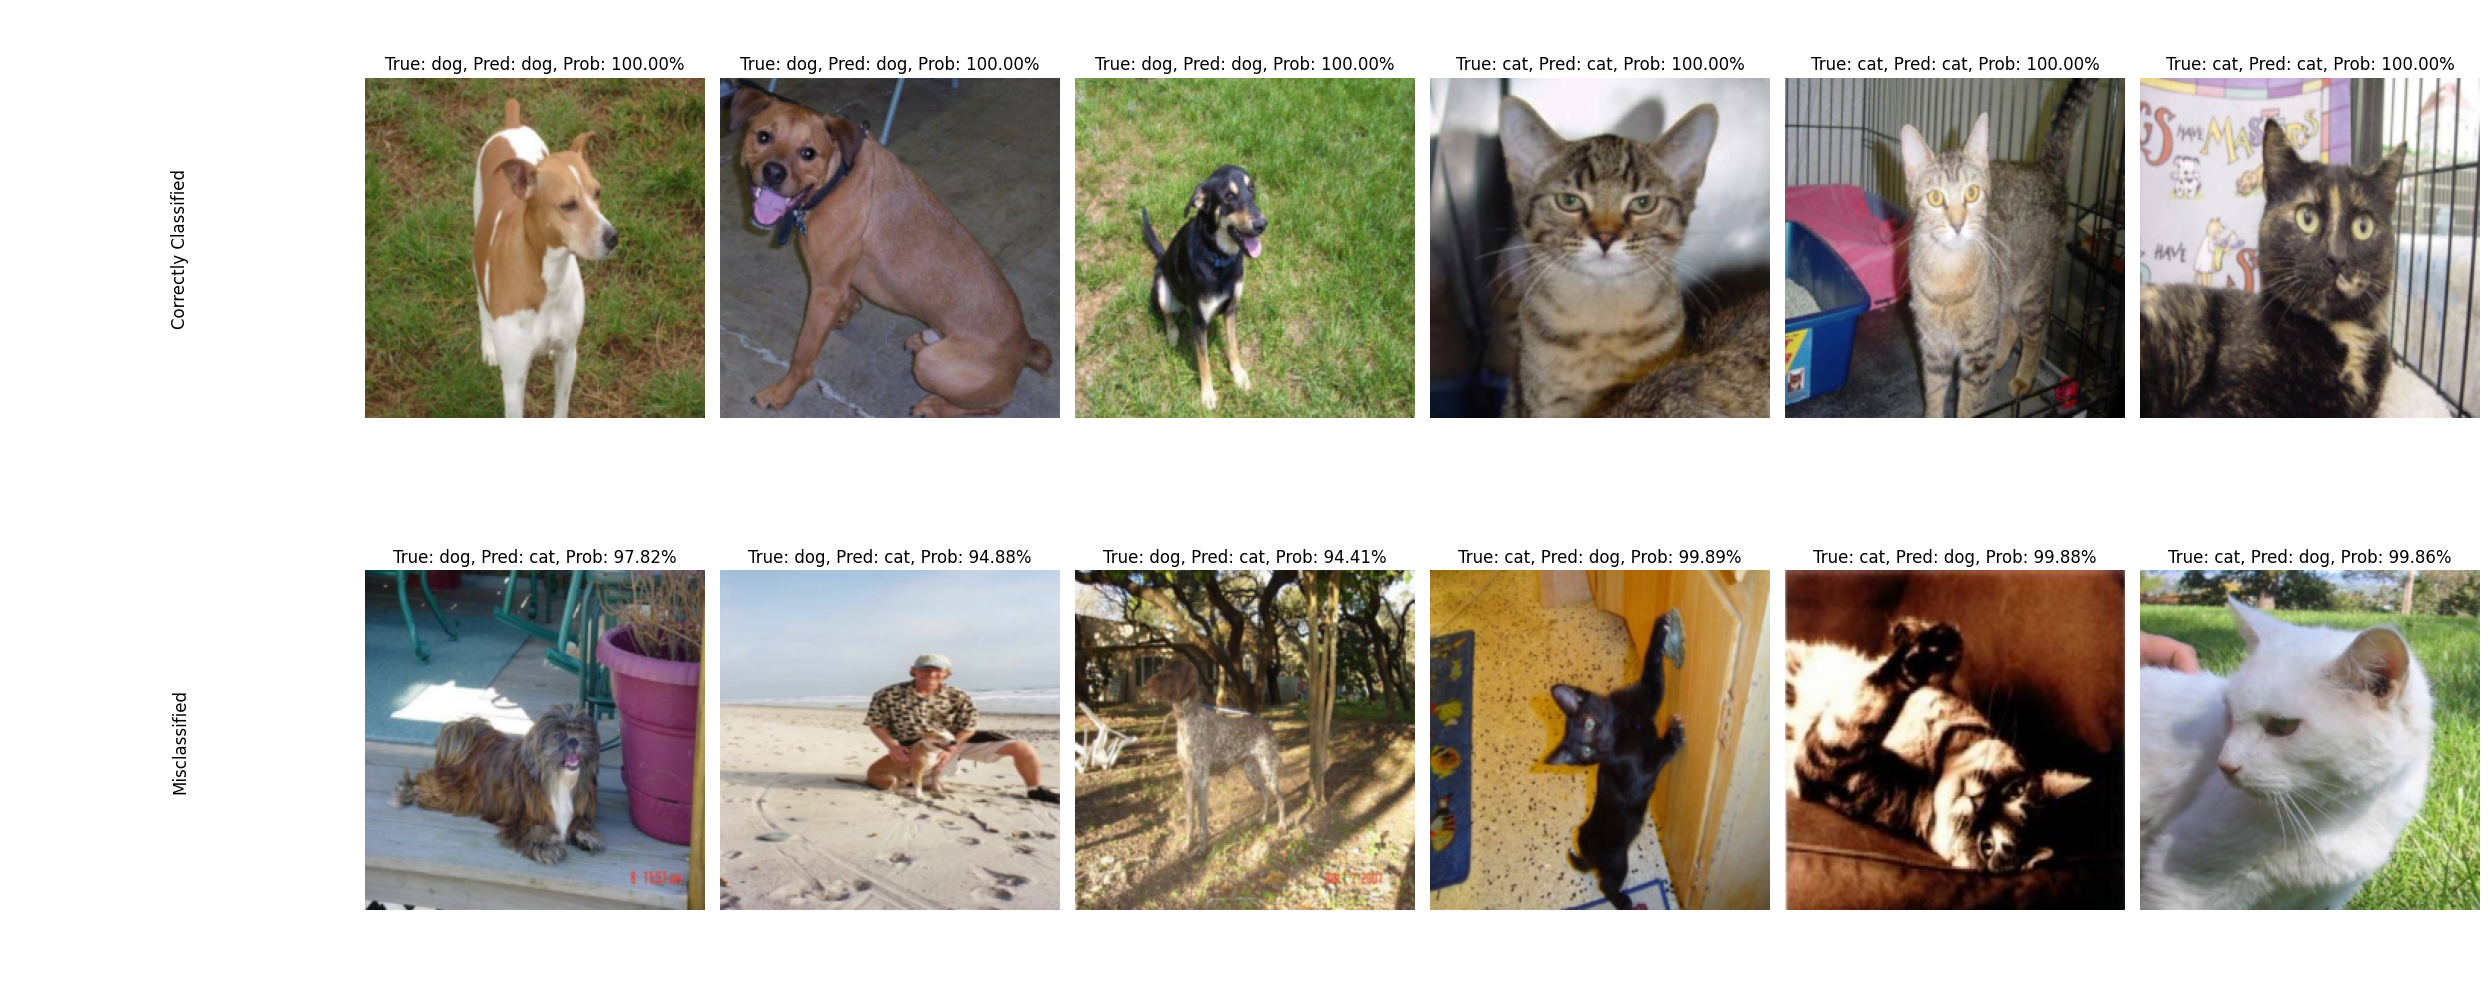
\includegraphics[width=1\textwidth]{figures/predict_images.png}
    \caption{Misclassified and correctly classified images.}
    \label{fig:prediction}
    \vspace*{-0.7cm}
\end{figure}

From the misclassified images, we see that may some more data augmentation could be applied to improve the model's performance.
For example, the cat that rotate its head by almost 90 degrees. Moreover, the model may be improved by adding more crop-scale augmentation.
\section{Pretrained Model (AlexNet)}
To see how good our model performs compared to a well-known model, we used the pretrained model 'AlexNet'.
This model is pretrained on the ImageNet dataset, which contains 1.2 million images and 1000 classes, also including cats and dogs.
However, to use the pretrained model for this binary classification task, the output layer is modified.
The results of the pretrained model after 20 epochs are shown in Figure \ref{fig:pretrained_model_results}.

\begin{figure}[H]
    \vspace*{-0.7cm}
    \centering
    % Subfigure 1:
    \subfloat[Loss and Accuracy scores using AlexNet.\label{fig:results_alexnet}]{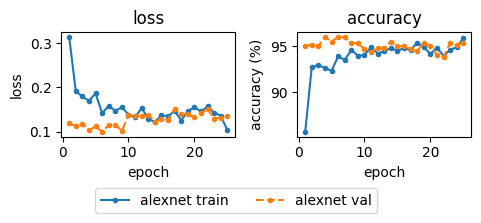
\includegraphics[width=0.4\textwidth]{figures/results_alexnet.png}}
    \hspace{0.4cm}
    \subfloat[Test Accuracy using AlexNet.\label{tab:alexnet}]{
        \raisebox{\height}{    
        \begin{tabular}{|c|}
            \hline
            \textbf{Test Accuracy} \\ \hline
            93.5\% \\ \hline
        \end{tabular}}}
    \caption{AlexNet results.}
    \label{fig:alexnet}
    \vspace*{-0.7cm}
\end{figure}


As expected the pretrained model performs sligtly better than our model.
However, AlexNet also is trained on a much larger dataset and has a lot more parameters ($\sim 57$ million) compared to our model ($\sim 21$ million).
\section{Conclusion}
We ended up with a model that has ?? results. The model we used was ?? with ?? layers having XX parameters. This result is pretty good, but it could be improved. It is worth noticing that some of the pictures are very hard to classify, like dog.1335 and dog.1395.

- compare results to pretrained model - why is the pretrained model better?


The model could have been improved in various ways.
First of all more training data would very likely improve the model a lot. In some of the pictures its very hard to see whether its a cat or a dog and its doubtful that the model would learn anything from the picture, so removing those pictures from the dataset would potentially help the model learn more meaningful features and also train faster.
We could have run epochs until the model began overfitting and then stopped at that point. If time was not a factor this is probably what we would have done.
We could have also experimented more with the different parameters like learning rate and weight decay. 
We could have tried even more data augmentations to see what works best. We only rotate the pictures up to 25 degrees, which means that the model as an example would have a hard time recognising pictures of animals upside down.


\subsection{Individual Contributions}
\begin{table}[H]
    \centering
    \begin{tabular}{|l|p{5cm}|p{5cm}|}
    \hline
                    & \textbf{Henrik Daniel Christensen} & \textbf{Frode Engtoft Johansen} \\ \hline
    \textbf{Code}   & - Base model \newline - Data Augmentation \newline - Regularization \newline - Pre-trained & \\ \hline
    \textbf{Report} & - Introduction \newline - Explorative Analysis \newline - Base Model \newline - Regularization \newline - Prediction \newline - Pretrained Model \newline - Conclusion & \\ \hline
    \end{tabular}
    \caption{Individual contributions.}
    \label{tab:individual_contributions}
\end{table}


%%%%%%%%%%%%%%%%%%%%%%%%%%%%%%%%%%%%%%%%%%%

%Appendices
\appendix
\section{Code}
hej
\includepdf[pages=1,scale=.85,pagecommand={\section{Notebook}\label{app:notebook}}]{../src/notebook.pdf}
\includepdf[pages=2-,scale=.85,pagecommand={}]{../src/notebook.pdf}

% \bibliographystyle{base/splncs04}
% \newpage
% \bibliography{base/references}
%%%%%%%%%%%%%%%%%%%%%%%%%%%%%%%%%%%%%%%%%%%
\end{document}